% Use xelatex to generate pdf file of this presentation

\documentclass{beamer}
\usepackage{roboto}
\usepackage[russian]{babel}
\usetheme{Copenhagen}

% Simple way to put a code listing to the slide
\usepackage{listings}

\usepackage{tikz}
\usepackage{graphicx}
  \logo{
\includegraphics[scale=0.1]{PostgresPro_logo}}
%Information to be included in the title page:
\title{Query plan freezing extension}
\subtitle{design,\ issues\ and\ lessons\ learned}
\author{Belyalov D., \underline{Lepikhov A.}, Rybakina A.}
\institute{Postgres Professional}
%\titlegraphic{\includegraphics[scale=0.05]{project_url}}
\date{2023}

% Add page numbers in footnote
\expandafter\def\expandafter\insertshorttitle\expandafter{%
  \insertshorttitle\hfill%
  \insertframenumber\,/\,\inserttotalframenumber}

\definecolor{lightlightgray}{gray}{0.9}

% -----------------------------

\begin{document}

\begin{frame}
\titlepage
   \tikz [remember picture,overlay]
    \node at
        ([yshift=2.0cm, xshift=-4.2cm]current page.center) 
        {
\includegraphics[scale=0.034]{project_logo}};
% Hi, My name is, I'm working in ... 
% I inntended to show here some results of our research dedicated to stabilizing query execution and reducing planning overhead.
% Here is the logo of our project, which is implemented in an extension as a tangible result which can give you some tool to find out new insights in this area. I will be glad to listen any feedback on that idea and tool.
% Execution routine can be destabilized by changings some settings, new data or just by autovaccum, which refreshes statistics on the data. Our purpose was to reduce risks of such actions.
\end{frame}

\begin{frame}[fragile]\frametitle{Self Introduction}
\begin{itemize}
  \item Specialist in Applied Mathematics graduated from Chelyabinsk State University in 2005
  \item Ph.D. in Computer Sciences (Distributed Databases) awarded at Moscow State University in 2008.
  \item Working in Postgres Professional as a Core Developer since 2017.
  \item Designed the Shardman project architecture on its earlier steps
  \item Worked on Multimaster project
  \item Working on various query optimization issues
\end{itemize}
% But at first I want to present myself, because it is my first speech outside motherland.
% I'm graduated in applied mathematics in 2005, awarded Ph.D. degree in 2009 at Moscow State University with Thesis dedicated to problem of load balancing during parallel query execution in database systems.
% First time I touched Postgres in 2007, it was a bit different DBMS these days. In PGPro I have been working since 2017. Since then I've designed Shardman - distributed DBMS based on postgres_fdw, foreign tables and partitioning machinery. Participated in Multimaster project and last two years working on query optimization issues.
\end{frame}

\begin{frame}[fragile]\frametitle{Who we are}
\begin{itemize}
  \item Research team, part of Postgres Professional, dealing with optimization issues
  \item Caused by the idea of sustainable coding
  \item Design enterprise and core features to improve the planner effectiveness
  \item Projects: Self-Join Removal, Asymmetric JOIN, Optimized Group-by, AQO, sr\_plan ...
% Our team is kind of R&D team inside PGPro. Inspired with ideas of resource effective coding and experiencing how much time and energy DBMS'es spend execution bad plans we started a set of project with main goal to reduce a number of optimization errors.
% Some of our projects you could already know, reading hackers mailing list or using PGPRO products, but some of the products, like replanning or adaptive join is still under development.
% But general idea still the same: create effective plans and provide a set of tools to manually correct mistakes if optimizer has failed.
\end{itemize}
\end{frame}

\begin{frame}[fragile]\frametitle{Plan freezing?}
\begin{columns}\begin{column}{0.6\textwidth}
\textbf{Reason 1:} \\
Don't optimize next time! \\
%\vspace{5mm}
\bigskip
pgbench:
\begin{itemize}
  \item With planning: $\approx$ 6000 tps
  \item Prepared statements: $\approx$ 7600 tps
\end{itemize}
% pgbench with prepared queries and not - reveals the potential
\end{column}
\begin{column}{0.4\textwidth}
  
\includegraphics[scale=0.7]{chalkboardlines}
\end{column}\end{columns}
% So, what's the stupid idea - freezing the plan? Working with OLTP loads and with a lot of clients who uses applications with auto-generated SQL code (Honestly at most one application - called 1C in Russia) we see, how much time DBMS spend to generate the same plan. Especially it make sense in the case of auto-generated queries where you can see a lot of joins, groupings, many generated indexes on one table for the only touching a few tuples in the databases.
% So, very often planning time outreaches execution time. Keeping in mind, that we do exactly the same job - it is harmful. Plan freezing don't solves this problem in general but can give a foundation for designing a technique for auto-freezing of queries like prepared statement switches to generic plan after a row of identical executions.
% One more driver here is foreign tables appended in a query through partitioning machinery. In the case of distributed execution we should plan each part of the query, executed on each foreign server which brings down total execution time of distributed query.
% Small part of the potential of this technique you can see, launching pgbench with and without preparation of statements. You can see, whateven in such unusual case we have about 30% speedup. So, that's the reason.
\end{frame}

\begin{frame}[fragile]\frametitle{Plan freezing?}
\begin{columns}\begin{column}{0.6\textwidth}
\textbf{Reason 2:} \\
Pin tweaked query plan into the plan cache:
\begin{itemize}
  \item Predictable execution time
  \item No planning surprises after minor upgrade
\end{itemize}
\end{column}
\begin{column}{0.4\textwidth}
  \begin{center}
    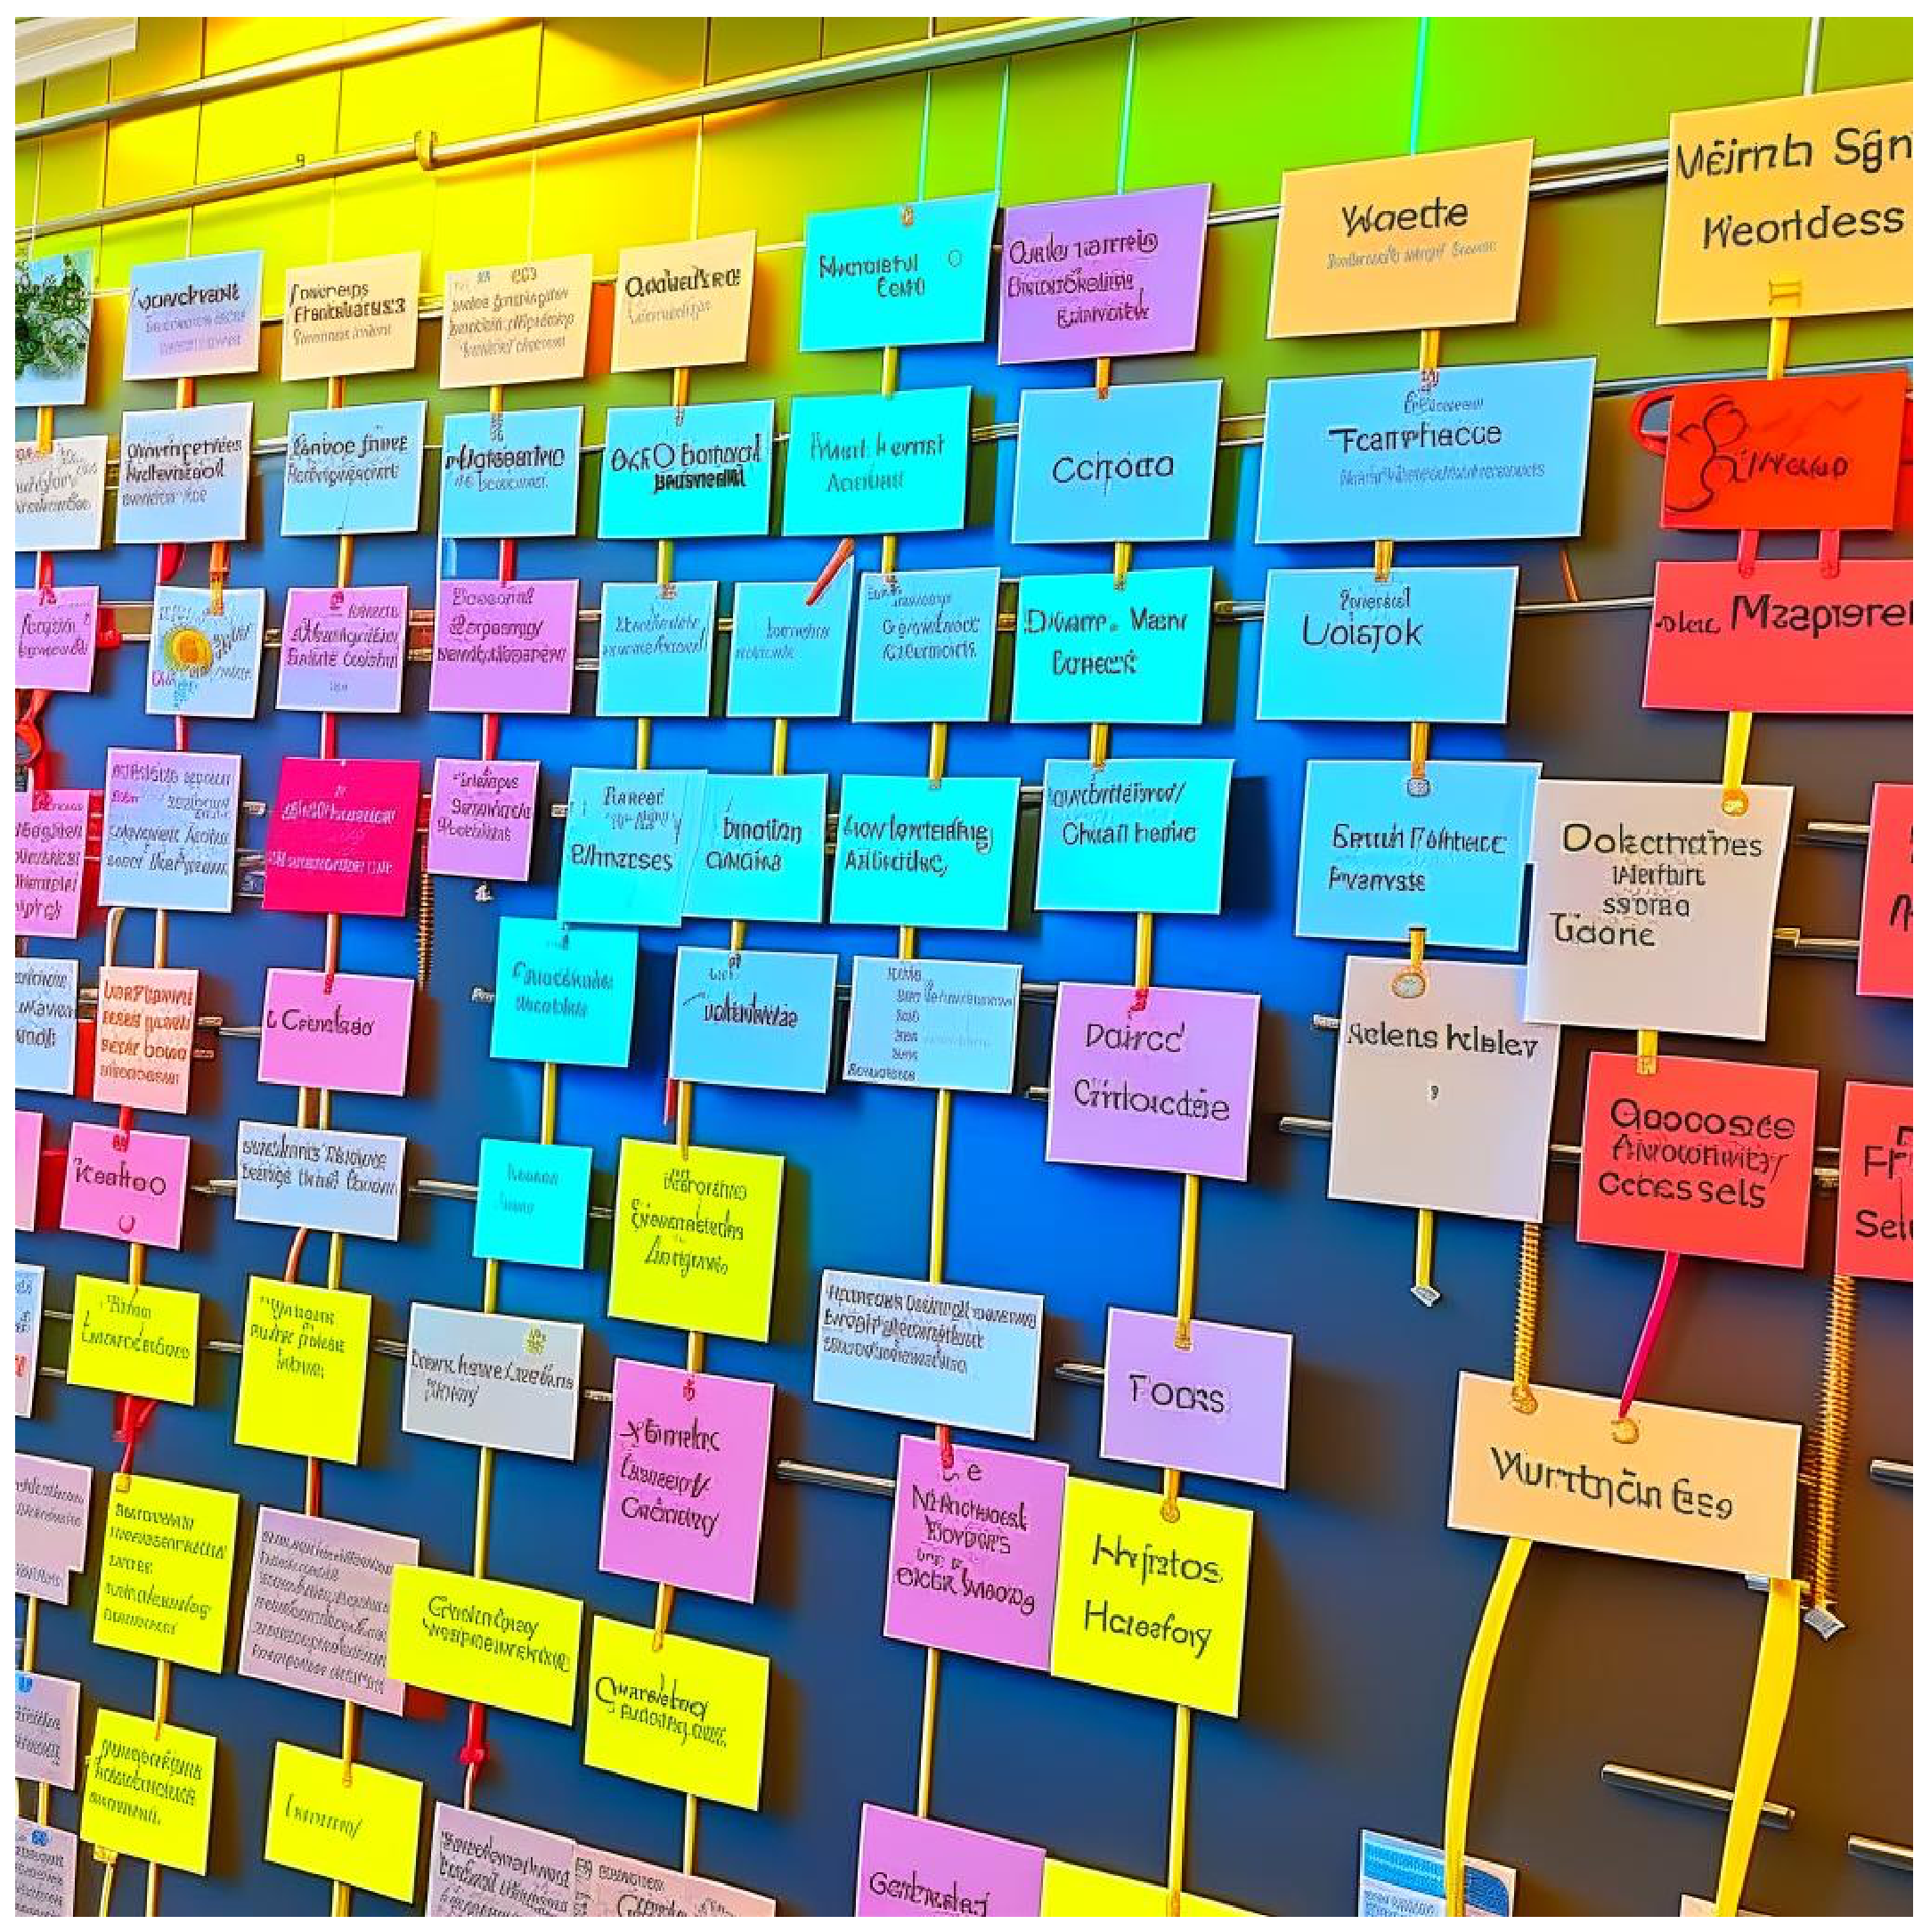
\includegraphics[scale=0.1]{stickers}
  \end{center}
\end{column}\end{columns}
% The next reason is much closer to the earth and caused by real enterprise requests.
% People want to have reliability in the sense of stable execution time. Maybe sometimes even more, than speeding up specific query.
% Sometimes subtle change in data set or statistics can trigger very different query plan and bring performance down. One of such examples is Join-Order Benchmark which contains hundred queries containing from 6 to 16 joins in one query. Executing them one by one you can realize, that repeating analysis of the unchanged tables causes huge performance flutter around 3-5 times in the value of execution time.
% One more thing here is unpredictable shifts after upgrades. Freezing technique can introduce some brand new style of safe migration: freeze plans before and unfreeze one-by-one after the upgrade. I guess, It looks like some Oracle users reported they do.
\end{frame}

\begin{frame}[fragile]\frametitle{Rationale}
% What is the origins of the idea to freeze plans
\begin{itemize}
  \item Stale statistics
  \item Imperfection of cost estimation algorithms
  \item Implicit functional dependencies between columns
\end{itemize}
% What is the reason for such harmful behaviour? Summarizing the experience I could classify it into three reasons.
% No one wants to do vacuum frequently. If you have queries which is quite complex, containing composite scan clauses and extract some small set of data from big tables, you should have actual statistics. Another way you have a risk to end up with non-optimal query plans. Query plan freezing here is a hack to delay vacuum or, at least, don't stuck into the problem unexpectedly.
% Second issue related to bugs, changes in cost model during pg_upgrade and other problems with the cost model we all know.
% And the most frequent last issue related to hidden functional dependencies. In practice it is the most awkward problem: we spend a lot of time to handle non-optimal plans here but at most can't do anything because PostgreSQL couldn't have tools to resolve it in common case.
% To briefly explain this issue, I want to show two cases.
\end{frame}

\begin{frame}[fragile]\frametitle{Functional Dependencies (overestimation)}
\lstset{language=sql, frame=none, tabsize=2, identifierstyle=\color{black},
  backgroundcolor=\color{lightlightgray},
  keywordstyle=\bfseries\color{green!40!black},showspaces=false, showtabs=false, showstringspaces=false}
\begin{lstlisting}[basicstyle=\footnotesize]
CREATE TABLE people (
  name          text,
  occupation    text,
  sex           boolean,
  region        text,
  is_vaccinated boolean
);
\end{lstlisting}
\begin{lstlisting}[basicstyle=\footnotesize]
SELECT * FROM people t1
WHERE occupation = 'Tractor Driver' AND sex = 'female'
/*
Seq Scan on people  (rows=1584) (actual rows=1)
   Filter: (is_woman AND (occupation = 'Tractor Driver'))
   Rows Removed by Filter: 99999
 */
\end{lstlisting}
\end{frame}

\begin{frame}[fragile]\frametitle{Functional Dependencies (underestimation)}
\lstset{language=sql, frame=none, tabsize=2, identifierstyle=\color{black},
  backgroundcolor=\color{lightlightgray},
  keywordstyle=\bfseries\color{green!40!black},showspaces=false, showtabs=false, showstringspaces=false}
\begin{lstlisting}[basicstyle=\footnotesize]
CREATE TABLE people (
  name          text,
  occupation    text,
  sex           boolean,
  region        text,
  is_vaccinated boolean
);
\end{lstlisting}
\begin{lstlisting}[basicstyle=\footnotesize]
SELECT * FROM people
WHERE region = 'Chelyabinsk' AND is_vaccinated;
/*
 Seq Scan on people  (rows=114) (actual rows=907)
   Filter: (is_vaccinated AND (region = 'Chelyabinsk'))
   Rows Removed by Filter: 99094
 */
\end{lstlisting}
\end{frame}

% Here we need some bridge from the planner slip-ups to the plan freezing
\begin{frame}[fragile]\frametitle{Our conjecture}
\begin{quote}
Unfortunate planning is inevitable [at least, for now]. Assuming someone or something could force the planner to generate a better plan, we should provide the tool to freeze the right solution for the subsequent executions.
\end{quote}
% Taking into account the whole experience we had, we formulated some conjecture. We assume the optimizer will miss. We don't know how to fix these errors - it would depend on the situation. But we give DBAs a tool to stick on the good plan.
% And, driven by this point of view we started to discover a way.
\end{frame}

\begin{frame}[fragile]\frametitle{Stick on the plan in the Plan Cache ?}
\begin{center}
  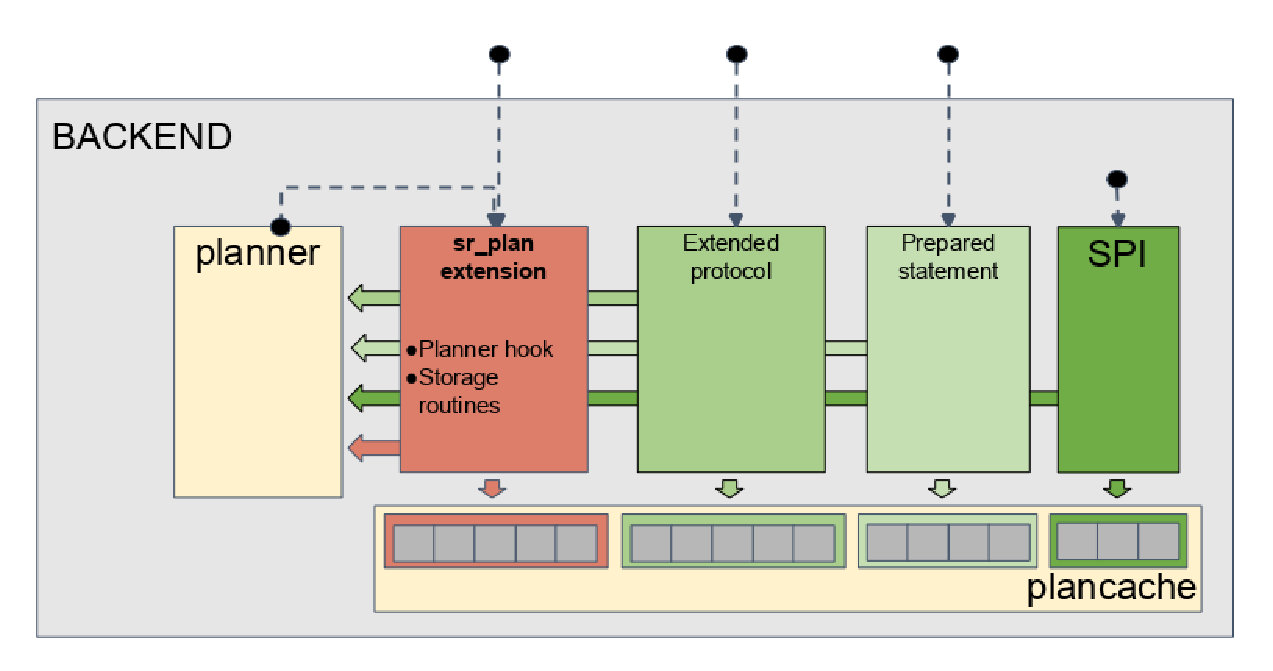
\includegraphics[width=\textwidth]{plancache_callers}
\end{center}
% At first, we found out that some features already stick on query plan. Here you see, that prepared statements, queries, sent by the extended protocol and some internal machinery called SPI use plan cache and can get a plan directly from the cache without planning.
% Here I need to explain a couple of terms. If we do the planning replacing parameters with using specific values of constants we call such plan as 'custom'. If we do the planning regardless of the specific parameter value, we call such a plan as generic.
% So, generic plan is designing without knowledge of parameter. If it uses in some filter or join, we can't exactly predict cardinality of such a scan and sometimes, optimizer generates suboptimal generic plans. So, custom plan most of the time is preferable than generic. 
% So, Prepared statements have a logic, according to which planner creates custom plan for the query. If after some attempts plan is the same, optimizer generates generic plan. If that plan is not too bad comparing to custom one, planner sticks on generic plan in plan cache and next time uses it without annoying planning. And it will use it until some ddl changes any object, touched by the plan and this plan will be dropped.
% extended protocol and SPI machinery utilizes the same logic.
% So, most of work already was done, we just needed to implement manual sticking of arbitrary query, provide cross-backend cache and disk storage to survive reboots.
\end{frame}

\begin{frame}[fragile]\frametitle{The sr\_plan extension}
\begin{columns}\begin{column}{0.8\textwidth}
\begin{itemize}
  \item Abbreviates \textbf{s}ave/\textbf{r}estore plan 
  \item Introduced in Postgres Pro Enterprise 15 (don\'t mix up with the extension sr\_plan existed up to PGPro Enterprise 13!)
  \item Freezes specific plan for a [parameterized] query
  % https://postgrespro.com/docs/enterprise/15/sr-plan
\end{itemize}
\end{column}
\begin{column}{0.2\textwidth}
  
\includegraphics[scale=0.7]{srplanqr}
\end{column}
\end{columns}
% And we have done that as a pure extension. We named it sr_plan. It abbreviates phrase save/restore plan. You already can play with that in our PGPro EE15.3, see QR code on the slide. What is it does? It gives you an UI using which you can freeze a plan for specific query, possible parameterized. I prefer to use term 'Statement' instead of 'Query', because in reality, remember triggers and rewriting rules which could be applied to your query - it maybe very different query that really will be executed. Sometimes.
% Although I've mentioned it is pure extension, it carries two slightly modified modules with no more than ten changed strings of code. The reason for this I'll explain  in the next slides.  
\end{frame}

\begin{frame}[fragile]\frametitle{How it works}
\begin{itemize}
  \item sr\_register\_query('SELECT ... WHERE x = \$1 AND y = 42', ...)
  \item sr\_plan\_freeze(srid)
  \item sr\_plan\_unfreeze(srid)
\end{itemize}
\begin{block}{Frozen plan have a special node in explain}
\begin{lstlisting}[basicstyle=\footnotesize]
                            QUERY PLAN          ------------------------------------------------
 Custom Scan (SRScan) (actual rows=1 loops=1)
   Frozen plan ID: 1
   ->  Aggregate (actual rows=1 loops=1)
      ->  Seq Scan on a (actual rows=10 loops=1)
            Filter: ((x = \$1) AND (y = 42)
\end{lstlisting}\end{block}
% The interface of the extension is very laconic. Mostly it is only two functions you need to use: register query and reeze it.
% As a first phase of freezing you need to register a query, passing to this function query string, parameterized if needed. It is local operation for the backend and no any impact on other backends of the instance you can do here.
% It just does the parsing procedure and saves parse tree of the query in some hash table and stick on the plan cache plan of each query whose parse tree will equal to this one.
% After execution of this function you can play with planner settings, statistics and so on until get satisfying plan.
% You can execute even EXPLAIN ANALYZE command for this query and can see that sr_plan catched your query by special Custom Node, inserted into the head of the plan. This node used for many reasons, such as passing specific values of query parameters, gathering statistics and so on. But the main thing here for user is the text string, named 'Frozen' or 'Registered' plan with ID of this plan in the extension storage.
% If the plan found you just call sr_plan_freeze routing and it sticks on your plan across all backends of the instance until you call unfreeze or some DDL make this plan invalid.
% Such 2-step freezing procedure designed because of architectural reasons ...
\end{frame}

\begin{frame}[fragile]\frametitle{Lesson 1}
\begin{columns}\begin{column}{0.5\textwidth}
In DBMS, the way from a query text to the plan is not straightforward.
\end{column}\begin{column}{0.5\textwidth}
\begin{center}
  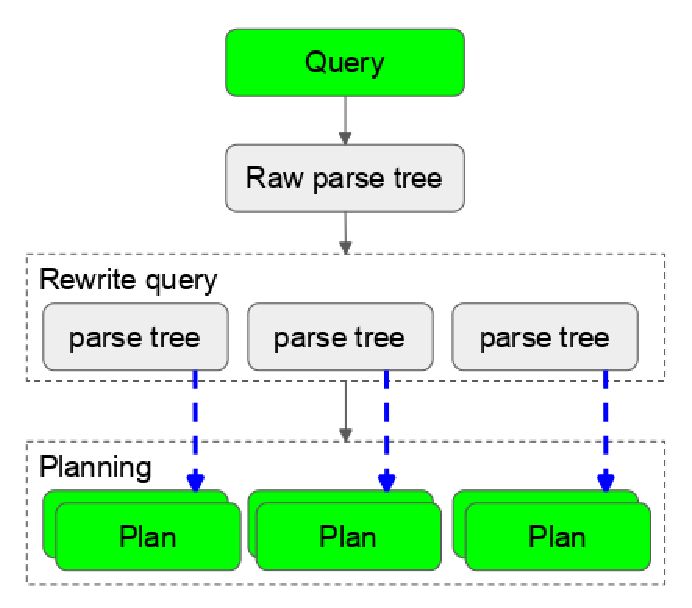
\includegraphics[scale=0.5]{query_planning_stages}
% The first lesson we've learnt since then is the query you have written isn't always which will be executed. It maybe looks strange, but rewriting rules, such as VIEWs, triggers or INSTEAD OF rules can change the real action. And because of definition of these rules can be changed from execution to execution, we can't base proof of plan usability on the query string.
% One query could trigger execution of a set of statements and it is not even enough to store raw parse tree and prove usability of the plan by the equality of stored and incoming tree.
% Discovering the way to match incoming query and the plan we found the only one option: stored and incoming parse trees must be equal or "almost" equal.
\end{center}\end{column}\end{columns}
\end{frame}

\begin{frame}[fragile]\frametitle{Lesson 2}
\begin{columns}\begin{column}{0.5\textwidth}
Only one way to prove applicability of the plan to the given query is to compare stored and incoming parse trees
\end{column}\begin{column}{0.5\textwidth}
  \begin{center}
    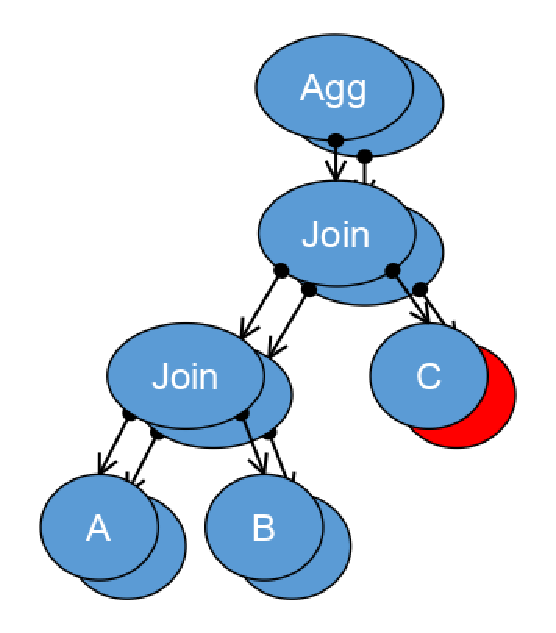
\includegraphics[scale=0.5]{compare_trees}
  \end{center}
\end{column}\end{columns}
% So, we implemented parse tree comparison technique which, of course, is more expensive than comparing text strings but have some pros - we don't mind and syntactic things like number of backspaces in certain places, using big or small letters, even full or short name of object. So, using tree comparison technique we covers more queries than even wanted at the commencement.
% You compare parse trees with oids of objects which is much more stable than names in textual form.
% Negative outcome is tree comparison procedure. As much details it will check as less queries you can execute with the frozen plan.
% Short example. Right now we use core function equal() to compare parse trees. It gives us portability and responsibility. But if you change any aliases of any column or a table, the extension wouldn't find frozen plan for such a query. So, here is a room for improvements.
% And it is the first module we slightly changed and carry as a part of the extension: we don't  compare aliases. So, the same query with different alias of a column can be executed with the same frozen plan.
\end{frame}

\begin{frame}[fragile]\frametitle{Lesson 3}
\begin{columns}\begin{column}{0.5\textwidth}
To make overhead admissible, we should have kind of parse tree signature - queryId
\end{column}\begin{column}{0.5\textwidth}
  \begin{center}
    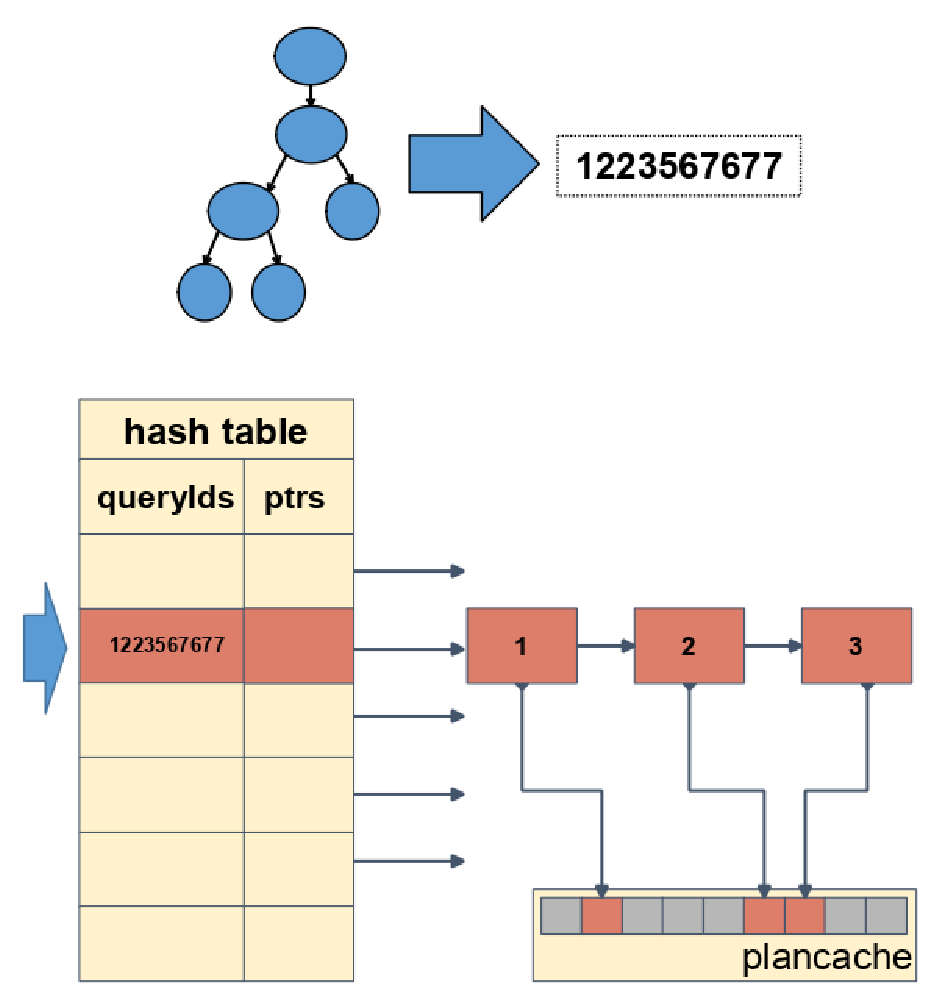
\includegraphics[scale=0.35]{queryid}
  \end{center}
\end{column}\end{columns}
% As you can already understand, comparing trees is too heavy operation. And if we needed to compare trees each other during the search we could can have only several frozen queries in the system. And it's the reason, why such an extension didn't invented before.
% To manage the overhead we need to classify queries into very small sets, normally containing only one parse tree. Like a signature.
% And such a feature had been introduced into the core with postgresql 13 and get improved since then. Now we have auto-generated code to sign parse tree. It gives quite good uniqueness of queries, sometimes even more than we really needed. 
% So, enabling the sr_plan you must enable queryId generation likewise in pg_stat_statements.
% All frozen queries we organized in lists with the same queryId - keep in mind that signature simplified by-design to reduce overheads. We find the list quickly by hash table, containing queryId as a key and pointer to the HEAD of the list.
% At this list we must compare incoming parse tree with each element until find full equality. But, according to our tests, usually we have only one element in such a list. And, as a result, minor overhead.
% At least we don't test a lot of queries with too simple or too complex trees. And usually complexity of the comparison is hidden under the complexity of query parsing.
\end{frame}

\begin{frame}[fragile]\frametitle{Lesson 4}
\begin{columns}\begin{column}{0.5\textwidth}
To apply plan freezing for parameterized queries we should '\textit{generalize}' the parse tree
\end{column}\begin{column}{0.5\textwidth}
  \begin{center}
    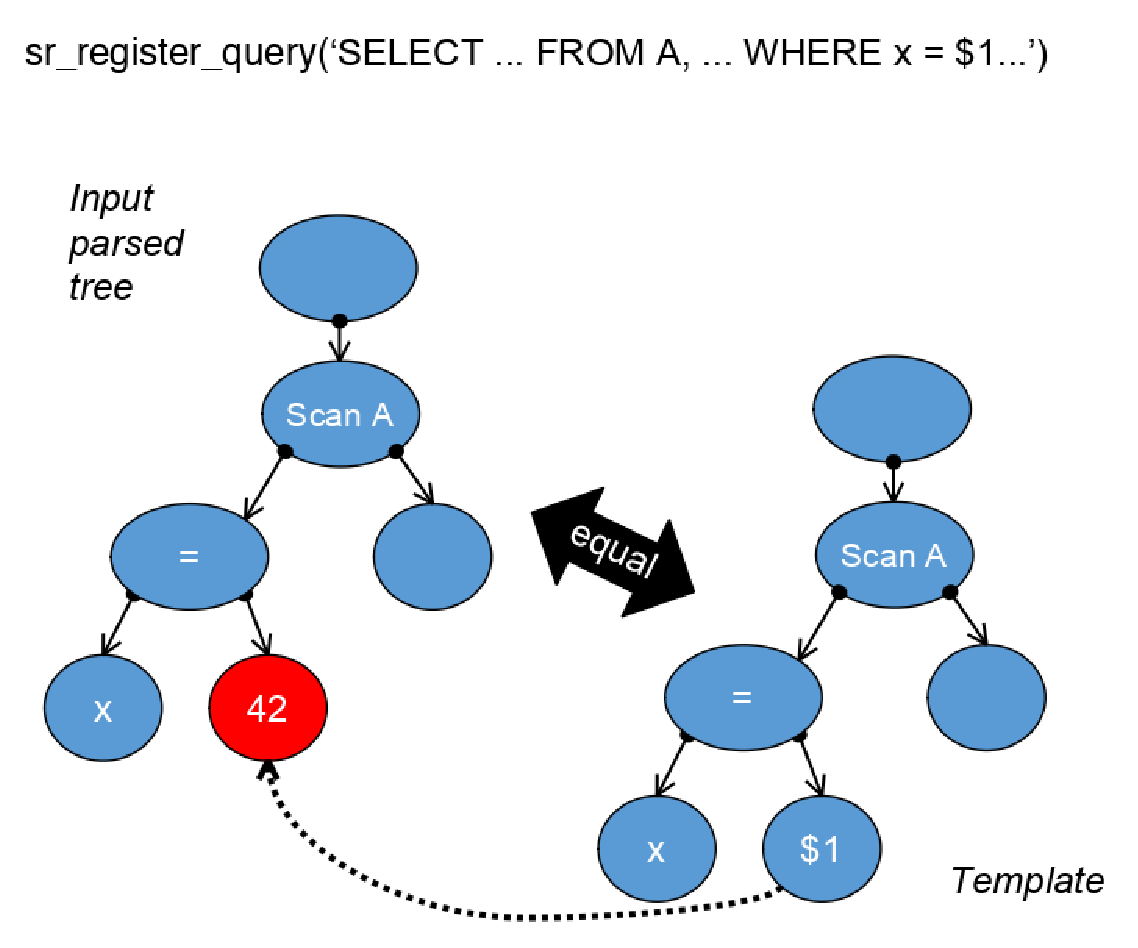
\includegraphics[scale=0.3]{tree_template}
  \end{center}
\end{column}\end{columns}
% The main challenge we struggled with was parameterization. We implemented the freezing of parameterized query statements, but it was challenging. An application sends a query with specific values of parameters. Because we have frozen a plan with parameters in expressions, core queryId and tree comparison aren't working. So, it's a reason why we slightly modified the upstream "queryId" code and maintained with the extension: To find a candidate frozen plan, we should generate a signature omitting the type of specific constant, thinking only about the type. Also, our implementation of queryId considers the only type of parameter. When we find a subset of candidates by query ID, the second phase takes place. To match the incoming parse tree and the frozen one, we must temporarily replace the constant node of the incoming parse tree in a given position with the parameter, the same as placed in that position in the frozen statement. After that, we can match these trees and prove the frozen plan's usability.
\end{frame}

\begin{frame}[fragile]\frametitle{Lesson 5}
\begin{columns}\begin{column}{0.4\textwidth}
The extension loading order matters
\end{column}\begin{column}{0.6\textwidth}
  \begin{center}
    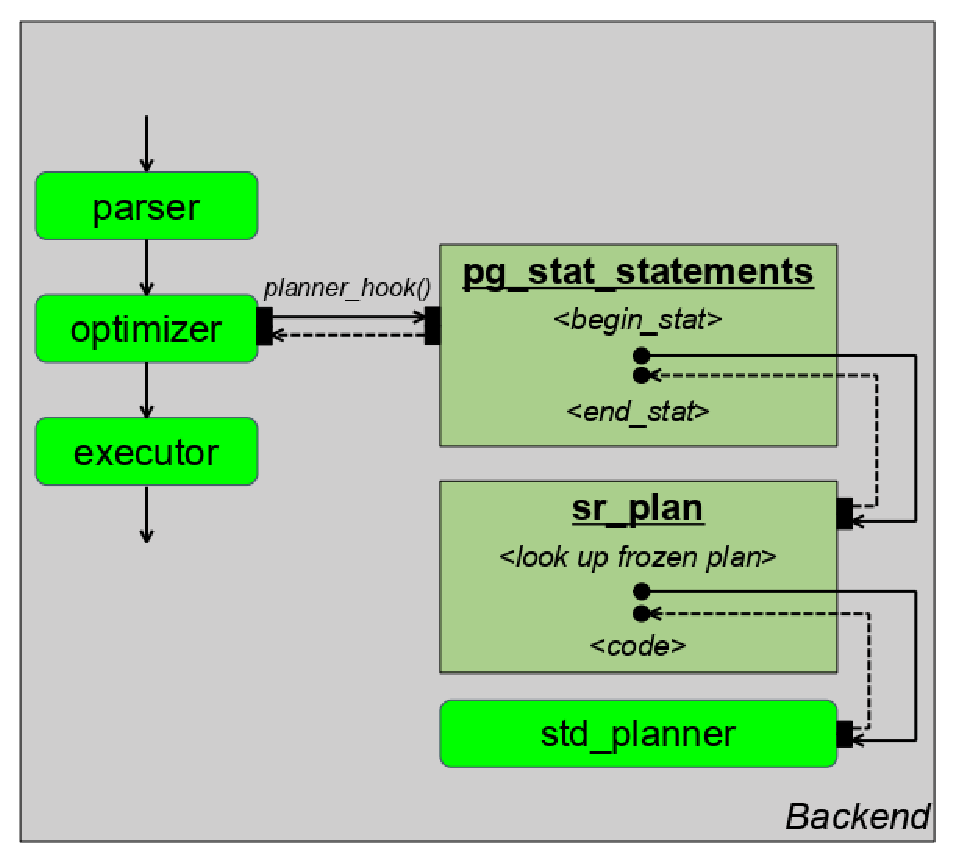
\includegraphics[scale=0.41]{hook_order}
  \end{center}
\end{column}\end{columns}
% One more lesson we learned during this work is the extension order. Trivial or not, but the order in which your extensions are loaded matters.
% For example, see this slide. We have two extensions here. They intercepted the planning hook and can provide some hints, an overall query plan, or just gather statistics. By convention, an extension should call the routine of a previously installed extension. So, here we place pg_stat_statements in the first position to take into account all actions that downstream extensions could do and summarize it after returning control from the routine call.
% sr_plan should stay the last in the queue of planner hooks. If it were not, the next extension in the queue would call the standard planner and spend time in the optimization module. It's a waste of time and CPU because sr_plan could just return the frozen plan. But if sr_plan doesn't have the next extension in the queue, it finds out the plan and returns it without planning at all.
% This is a kind of instability we found in Postgres extensions. Usually, in the extensions that intercept the planner hook, it makes sense for any other modules, too.
\end{frame}

\begin{frame}[fragile]\frametitle{Points of overhead}
\begin{columns}\begin{column}{0.5\textwidth}
\begin{itemize}
  \item Parse tree comparison
  \item Plan invalidation
  \begin{itemize}
    \item Per-backend cache invalidation
    \item Disc storage sync
    \item Transactional issues
  \end{itemize}
\end{itemize}
\end{column}\begin{column}{0.5\textwidth}
  \begin{center}
    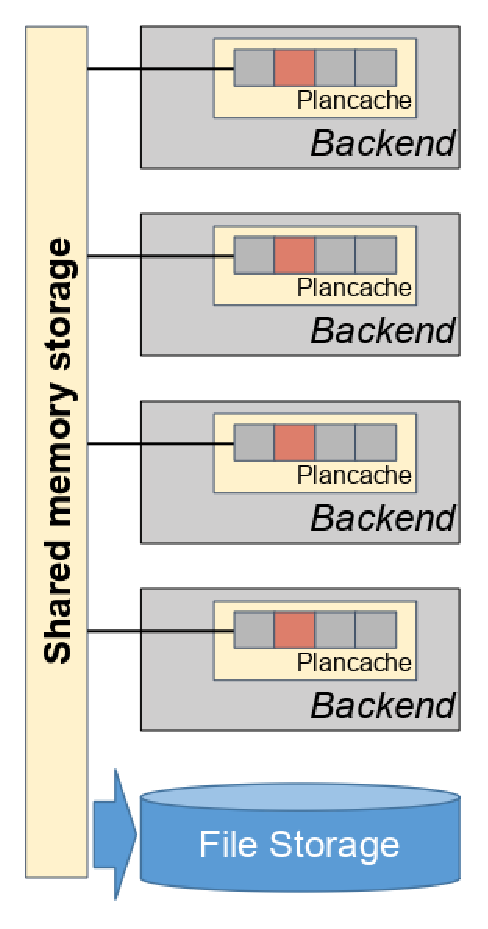
\includegraphics[scale=0.4]{plancache_invalidation}
  \end{center}
\end{column}\end{columns}
% Couple words about overheads.
% We discussed one obvious overhead related to proof of the frozen plan applicability. It is inevitable overhead and we reduce it down to fraction of percent by usage of queryId signatures.
% One more point of overhead here is synchronization of local plan caches and invalidation procedure:
% In the case, we add new frozen statement it must be sent to shared memory and spreaded across all backends registered in database to which frozen plan is related.
% This procedure have caveats because of MVCC, another backend could not have the same objects: relations, functions etc, which already (or still) have freezing backend.
% So, we introduced some 'validation' procedure according to which we examine this frozen statement. Of course it doing in the subtransaction, we build parse tree, compare it with frozen one, serialize/deserialize query plan and check all indexes used in this plan. It is heavy operation, but we keep in mind that DDL which changes the schema is not frequent, usually. So, keep in mind this fact, when use sr_plan.
% One more point of overhead is disk writing procedures. We use files to store frozen plans. So, it isn't cached and writes serially, writing down all frozen plans one-by-one. So, each freeze/unfreeze procedure more heavy, than before and this cost increases with growth of number of frozen plans.
\end{frame}

\begin{frame}[fragile]\frametitle{Freeze pgbench}
\begin{block}{Freezing procedure}
\lstset{language=sql, frame=none, identifierstyle=\color{black},
  keywordstyle=\bfseries\color{green!40!black},showspaces=false, showtabs=false, showstringspaces=false,}
\begin{lstlisting}[basicstyle=\footnotesize]
SELECT srid FROM sr_register_query('
  SELECT abalance FROM pgbench_accounts
  WHERE aid = $1', 'int')  \gset
SELECT abalance FROM pgbench_accounts WHERE aid = 1;
SELECT sr_plan_freeze(:srid);
\end{lstlisting}
\end{block}
\begin{columns}\begin{column}{0.4\textwidth}
\begin{lstlisting}[basicstyle=\tiny]
UPDATE pgbench_accounts ...
UPDATE pgbench_tellers ...
UPDATE pgbench_branches ...
INSERT INTO pgbench_history ...
\end{lstlisting}
\end{column}\begin{column}{0.6\textwidth}
\begin{itemize}
  \item With planning: $\approx$ 6000 tps
  \item Frozen statements: $\approx$ 6500 tps
\end{itemize}
\end{column}\end{columns}
% To demonstrate how it works and what you can do in a minute I have frozen pgbench queries. All of them. You remember, may be - here we have 3 updates, one insertion and one select query. All of them have trivial query plan and in reality such a freezing don't make a lot of sense. But for us it is sort of zero point. Overhead here shouldn't  overweigh efefct of freezing. Of course, we set the extension as a last extension in the list and no additional plannings needed at all.
% Here you can see psql commands how I freeze SELECT query. For other queries the same technique is used. Launching the pgbench test with 5 threads 5 clients on my laptop I've got about 8% performance gain. It is may be too small profit, but the purpose for this feature a bit different. So, even with 5 frozen queries and pgbench test we don't loose performance. And that's OK, I think.
\end{frame}

\begin{frame}[fragile]\frametitle{The future}
\begin{itemize}
  \item Global prepared statements
  \item Detect bad plan and try something different
  \item Plan transfer procedure
% Let me tell a bit about the future of this extension.
% It is made as an enterprise solution occasionally. The main purpose is different. We have been looking at this extension as a playground for much more interesting Core and EE features.
% GPS - it looks like we can move stored plan from shmem to the system catalog, to make it happens. Here is, of course, a lot of work with plan invalidation issues. But still, it is a good tool.
% It is kind of machinery for searching for better plan if it has detected that current plan is too bad. Imagine, after the query execution you check real number of tuples produces in each node of query plan and compare with the planned ones. If you see, that  cumulative error is high, you can try to signal DBA about it and they have a chance to improve the query by hand or just experimenting with extended statistics etc. The machinery I described here is a base to invent such new features.
% The method of plan usage proof can be used for safe transfer to another instance with the BKI. Using subtransactions we can imagine such external tool for dump/restore of plans.
\end{itemize}
\end{frame}

\begin{frame}
\begin{center}
\begin{center}

\includegraphics[scale=0.1]{project_logo}
\end{center}
\huge{Questions ?}
\end{center}
\end{frame}

\end{document}
